\documentclass[final,hyperref={pdfpagelabels=false}]{beamer}
\mode<presentation>
  {
  %  \usetheme{Berlin}
  \usetheme{PotsdamPoster}
  }
\usepackage{amsmath,amsthm, amssymb, latexsym}
\boldmath
\usepackage[english]{babel}
\usepackage[latin1]{inputenc}
\usepackage[orientation=portrait,size=a0,scale=1.6,debug]{beamerposter}

\usepackage{listings}

\setbeamersize{text margin left=2cm, sidebar width left = 0cm, text margin right = 2cm}

\newcommand{\e}{\mathrm{e}}
\newcommand{\op}[1]{\hat #1}
\newcommand{\rmd}{\mathrm{d}}
\newcommand{\mean}[1]{\langle #1 \rangle}

\newcommand\T{\rule{0pt}{2.0ex}}
\newcommand\B{\rule[-1.2ex]{0pt}{0pt}}

\title{Solving ODEs in C++}
\author{Karsten Ahnert and Mario Mulansky}
\institute[Uni Potsdam]{Institute of Physics and Astronomy, University of Potsdam}
\date{\today}
\renewcommand{\webaddress}{http://www.odeint.com}
\renewcommand{\email}{karsten.ahnert@gmx.de, mario.mulansky@gmx.net}
\renewcommand{\reference}{University of Potsdam, AmbroSys GmbH}


%%%%% C++ Style

\definecolor{dark-gray}{gray}{0.15}
\definecolor{light-gray}{gray}{0.8}
\definecolor{lighter-gray}{gray}{0.9}

\definecolor{dark-green}{rgb}{0,0.4,0}
\definecolor{dark-red}{rgb}{0.2,0,0}

\lstset{
         basicstyle=\small\ttfamily, % Standardschrift
         %numbers=left,               % Ort der Zeilennummern
         numberstyle=\tiny,          % Stil der Zeilennummern
         %stepnumber=2,               % Abstand zwischen den Zeilennummern
         numbersep=0pt,              % Abstand der Nummern zum Text
         tabsize=2,                  % Groesse von Tabs
         extendedchars=true,         %
         breaklines=true,            % Zeilen werden Umgebrochen
         frame=single,         
         backgroundcolor=\color{lighter-gray},
         tabsize=2,
         keywordstyle=\color{dark-green},
         identifierstyle=,
         commentstyle=\color{dark-gray}\normalfont\rmfamily\itshape,
         stringstyle=\color{dark-red},
         showspaces=false,           % Leerzeichen anzeigen ?
         showtabs=false,             % Tabs anzeigen ?
         xleftmargin=10pt,
         xrightmargin=10pt,
         framexleftmargin=5pt,
         framexrightmargin=5pt,
         framexbottommargin=4pt,
         language=c++,
         showstringspaces=false      % Leerzeichen in Strings anzeigen ?        
 }
\lstloadlanguages{C++}

  %%%%%%%%%%%%%%%%%%%%%%%%%%%%%%%%%%%%%%%%%%%%%%%%%%%%%%%%%%%%%%%%%%%%%%%%%%%%%%%%%5

%\let\raggedright\relax

\begin{document}
  \begin{frame}[fragile]{} 

\vspace{-2cm}

\begin{columns}[t]
  \begin{column}{0.32\linewidth}
    \begin{blockwh}{General}{10.5cm}
      \begin{itemize}
	\item Boost library (since Boost v1.53)
	\item Fully Open Source (Boost license)
	\item Modern and generic C++ code
	\item Highly flexible
	\item Fast
      \end{itemize}
    \end{blockwh}
    
    \vspace{1cm}
    
    \begin{blockwh}{Includes}{23.35cm}
      \begin{itemize}
	\item Runge-Kutta schemes:
	\begin{itemize}
	  \item Runge-Kutta4
	  \item Runge-Kutta-Dopri5
	  \item Runge-Kutta-Cash-Karp
	  \item Runge-Kutta78
	\end{itemize}
	\item Step-Size Control
	\item Dense Output
	\item Multistep Methods (Adams-Bashforth)
	\item Bulirsch-Stoer
	\item Implicit Rosenbrock scheme
      \end{itemize}
      \vspace{1em}
      \begin{itemize}
       \item High-level integrate routines
       \item Iterator abstraction
      \end{itemize}

    \end{blockwh}
  \end{column}

\begin{column}{0.67\linewidth}
    \begin{blockwh}{Lorenz Example -- 30 lines of code}{41.7cm}
    \begin{lstlisting}
#include <iostream>
#include <boost/array.hpp>
#include <boost/numeric/odeint.hpp>

using namespace std;
using namespace boost::numeric::odeint;

const double sigma = 10.0;
const double R = 28.0;
const double b = 8.0 / 3.0;

typedef boost::array< double , 3 > state_type;

void lorenz( const state_type &x , state_type &dxdt , double t )
{
    dxdt[0] = sigma * ( x[1] - x[0] );
    dxdt[1] = R * x[0] - x[1] - x[0] * x[2];
    dxdt[2] = -b * x[2] + x[0] * x[1];
}

void write_lorenz( const state_type &x , const double t )
{
    cout << t << '\t' << x[0] << '\t' << x[1] << '\t' << x[2] << endl;
}

int main(int argc, char **argv)
{
    state_type x = { 10.0 , 1.0 , 1.0 }; // initial conditions
    integrate( lorenz , x , 0.0 , 25.0 , 0.1 , write_lorenz );
}
    \end{lstlisting}
    \end{blockwh}
  \end{column}

\end{columns}

\vspace{0.5cm}

\begin{columns}[t]
  \begin{column}{0.495\linewidth}
    \begin{blockwh}{Structure}{26.0cm}
      \centering
      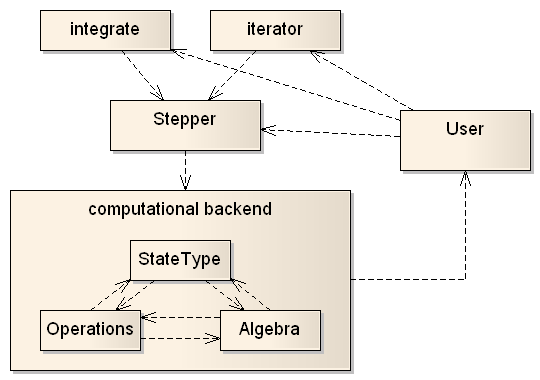
\includegraphics[width=0.95\textwidth]{odeint_modularization.png}
    \end{blockwh}
  \end{column}

  \begin{column}{0.495\linewidth}
    \begin{blockwh}{Independent Algorithms}{24.5cm}
      \begin{itemize}
       \item Separate algorithm from computational details
       \item Container-independent implementation
       \item Memory management detached from algorithms
       \item Each part interchangeable by the user
      \end{itemize}
      \vspace{1em}
      {\large$\longrightarrow$ Incredible Flexibility:}
      \vspace{.5em}
      \begin{itemize}
       \item Supports any container as state type
       \item Natively supports complex numbers
       \item Works with many linear algebra libraries: MTL, uBlas, eigen
       \item \textbf{Runs on GPUs} (via Cuda/Thrust or OpenCL/vexCL)
       \item Can be used with multi-precision types (e.g.\ Boost.Multiprecision)
       \item Easily extendable to run with your own state type, e.g.\ graphs or complex networks
       \item Parallelized backends available soon (OpenMP, MPI, HPX)
      \end{itemize}

    \end{blockwh}
  \end{column}

\end{columns}

\begin{columns}[t]

\begin{column}{0.495\linewidth}
    \begin{blockwh}{Performance -- Lorenz System, RK4}{15.5cm}
     \centering
     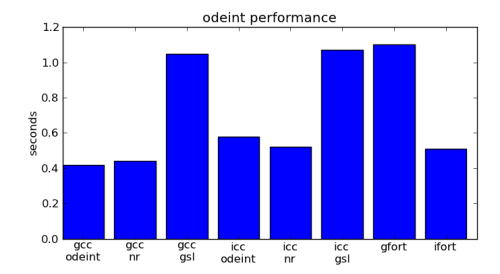
\includegraphics[height=17.1cm]{performance.png}
    \end{blockwh}
  \end{column}

  \begin{column}{0.24\linewidth}
    \begin{blockwh}{Details}{15.5cm}
     \begin{itemize}
      \item Modularization by Generic Programming
      \item No virtual function calls
      \item Metaprogramming to generate Runge-Kutta schemes
      \item Extensive unit tests
      \item Reviewed by top C++ programmers (Boost community)
     \end{itemize}
    \end{blockwh}
  \end{column}
  
  \begin{column}{0.24\linewidth}
    \begin{blockwh}{Users}{15.5cm}
    \begin{itemize}
     \item \textbf{NetEvo} {\small (Dynamical Networks)}\\[.5em]
     \item \textbf{OMPL} {\small (Motion Planning)}\\[.5em]
     \item \textbf{icicle} {\small (Cloud Modeling)}\\[.5em]
     \item \textbf{Score} {\small (commercial SPH)}\\[.5em]
     \item \textbf{VLE} {\small (Virtual Laboratory)}\\[.5em]
     \item Several research groups
    \end{itemize}
    \end{blockwh}
  \end{column}
\end{columns}
\vglue-2cm
\end{frame}

\end{document}